% This file was created with tikzplotlib v0.10.1.
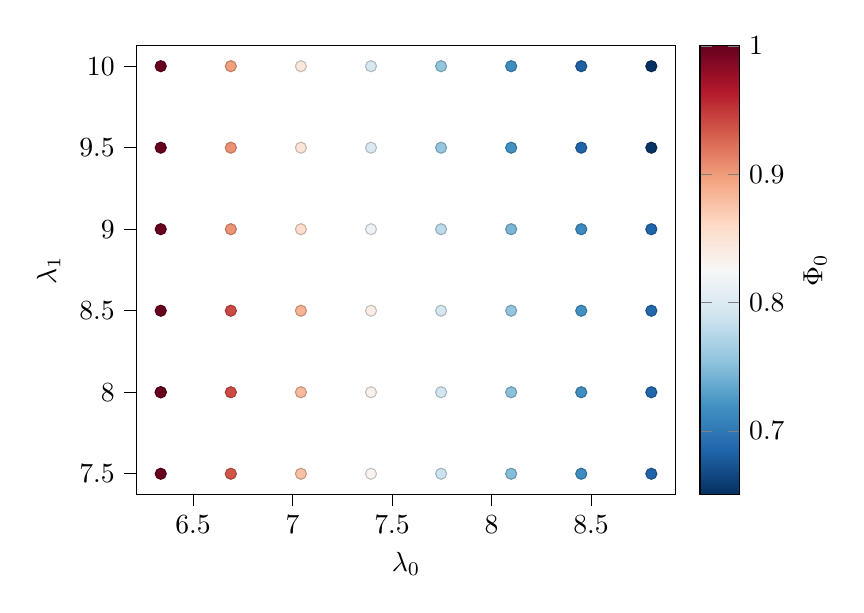
\begin{tikzpicture}

\definecolor{darkgray176}{RGB}{176,176,176}

\begin{axis}[
colorbar,
colorbar style={ylabel={$\Phi_{0}$}},
colormap={mymap}{[1pt]
  rgb(0pt)=(0.0196078431372549,0.188235294117647,0.380392156862745);
  rgb(1pt)=(0.129411764705882,0.4,0.674509803921569);
  rgb(2pt)=(0.262745098039216,0.576470588235294,0.764705882352941);
  rgb(3pt)=(0.572549019607843,0.772549019607843,0.870588235294118);
  rgb(4pt)=(0.819607843137255,0.898039215686275,0.941176470588235);
  rgb(5pt)=(0.968627450980392,0.968627450980392,0.968627450980392);
  rgb(6pt)=(0.992156862745098,0.858823529411765,0.780392156862745);
  rgb(7pt)=(0.956862745098039,0.647058823529412,0.509803921568627);
  rgb(8pt)=(0.83921568627451,0.376470588235294,0.301960784313725);
  rgb(9pt)=(0.698039215686274,0.0941176470588235,0.168627450980392);
  rgb(10pt)=(0.403921568627451,0,0.12156862745098)
},
point meta max=1,
point meta min=0.650743582033671,
tick align=outside,
tick pos=left,
x grid style={darkgray176},
xlabel={\(\displaystyle \lambda_{0}\)},
xmin=6.2147887314, xmax=8.9260563366,
xtick style={color=black},
y grid style={darkgray176},
ylabel={\(\displaystyle \lambda_{1}\)},
ymin=7.375, ymax=10.125,
ytick style={color=black}
]
\addplot [
  colormap={mymap}{[1pt]
  rgb(0pt)=(0.0196078431372549,0.188235294117647,0.380392156862745);
  rgb(1pt)=(0.129411764705882,0.4,0.674509803921569);
  rgb(2pt)=(0.262745098039216,0.576470588235294,0.764705882352941);
  rgb(3pt)=(0.572549019607843,0.772549019607843,0.870588235294118);
  rgb(4pt)=(0.819607843137255,0.898039215686275,0.941176470588235);
  rgb(5pt)=(0.968627450980392,0.968627450980392,0.968627450980392);
  rgb(6pt)=(0.992156862745098,0.858823529411765,0.780392156862745);
  rgb(7pt)=(0.956862745098039,0.647058823529412,0.509803921568627);
  rgb(8pt)=(0.83921568627451,0.376470588235294,0.301960784313725);
  rgb(9pt)=(0.698039215686274,0.0941176470588235,0.168627450980392);
  rgb(10pt)=(0.403921568627451,0,0.12156862745098)
},
  only marks,
  scatter,
  scatter src=explicit
]
table [x=x, y=y, meta=colordata]{%
x  y  colordata
6.338028168 7.5 1.0
6.338028168 8 1.0
6.338028168 8 1.0
6.338028168 8.5 1.0
6.338028168 9 1.0
6.338028168 9.5 1.0
6.690140844 7.5 0.9352172172903122
6.690140844 8 0.9398969961392923
6.690140844 8.5 0.941017092226102
6.690140844 9 0.9039342822812801
6.690140844 9.5 0.9049530932442569
6.690140844 10 0.8981964631416062
7.04225352 7.5 0.8781161980003005
7.04225352 8 0.8819290285525373
7.04225352 8.5 0.8861252897014062
7.04225352 9 0.857702921029864
7.04225352 9.5 0.8481285516998385
7.04225352 10 0.8442166029162511
7.394366196 7.5 0.8304842490571266
7.394366196 8 0.833944204825183
7.394366196 8.5 0.8381320508934788
7.394366196 9 0.8162181234972332
7.394366196 9.5 0.8001831135211429
7.394366196 10 0.7973008580533767
7.746478872 7.5 0.7879175578983306
7.746478872 8 0.7912063775889707
7.746478872 8.5 0.7947808504070476
7.746478872 9 0.7789912510897511
7.746478872 9.5 0.7571199279539385
7.746478872 10 0.7556778512005778
8.098591548 7.5 0.7500834946277738
8.098591548 8 0.7525673745423506
8.098591548 8.5 0.7559294236212115
8.450704224 7.5 0.7154304516678646
8.450704224 8 0.7172184818029398
8.450704224 8.5 0.7192164069902506
8.8028169 8 0.6853258962459483
8.8028169 8.5 0.6874089836536891
8.098591548 9 0.7450016538381432
8.098591548 9.5 0.7187458630630492
8.098591548 10 0.7165440378366962
8.450704224 9 0.7135642078749624
8.450704224 9.5 0.6841027227217337
8.450704224 10 0.6816787378131463
8.8028169 9 0.6842909781673083
8.8028169 9.5 0.6528036417354933
8.8028169 10 0.6507435820336711
6.338028168 10 1.0
8.8028169 7.5 0.6840480413287581
};
\end{axis}

\end{tikzpicture}
